% Options for packages loaded elsewhere
\PassOptionsToPackage{unicode}{hyperref}
\PassOptionsToPackage{hyphens}{url}
\PassOptionsToPackage{dvipsnames,svgnames,x11names}{xcolor}
%
\documentclass[
  letterpaper,
  DIV=11,
  numbers=noendperiod]{scrartcl}

\usepackage{amsmath,amssymb}
\usepackage{iftex}
\ifPDFTeX
  \usepackage[T1]{fontenc}
  \usepackage[utf8]{inputenc}
  \usepackage{textcomp} % provide euro and other symbols
\else % if luatex or xetex
  \usepackage{unicode-math}
  \defaultfontfeatures{Scale=MatchLowercase}
  \defaultfontfeatures[\rmfamily]{Ligatures=TeX,Scale=1}
\fi
\usepackage{lmodern}
\ifPDFTeX\else  
    % xetex/luatex font selection
\fi
% Use upquote if available, for straight quotes in verbatim environments
\IfFileExists{upquote.sty}{\usepackage{upquote}}{}
\IfFileExists{microtype.sty}{% use microtype if available
  \usepackage[]{microtype}
  \UseMicrotypeSet[protrusion]{basicmath} % disable protrusion for tt fonts
}{}
\makeatletter
\@ifundefined{KOMAClassName}{% if non-KOMA class
  \IfFileExists{parskip.sty}{%
    \usepackage{parskip}
  }{% else
    \setlength{\parindent}{0pt}
    \setlength{\parskip}{6pt plus 2pt minus 1pt}}
}{% if KOMA class
  \KOMAoptions{parskip=half}}
\makeatother
\usepackage{xcolor}
\setlength{\emergencystretch}{3em} % prevent overfull lines
\setcounter{secnumdepth}{-\maxdimen} % remove section numbering
% Make \paragraph and \subparagraph free-standing
\ifx\paragraph\undefined\else
  \let\oldparagraph\paragraph
  \renewcommand{\paragraph}[1]{\oldparagraph{#1}\mbox{}}
\fi
\ifx\subparagraph\undefined\else
  \let\oldsubparagraph\subparagraph
  \renewcommand{\subparagraph}[1]{\oldsubparagraph{#1}\mbox{}}
\fi

\usepackage{color}
\usepackage{fancyvrb}
\newcommand{\VerbBar}{|}
\newcommand{\VERB}{\Verb[commandchars=\\\{\}]}
\DefineVerbatimEnvironment{Highlighting}{Verbatim}{commandchars=\\\{\}}
% Add ',fontsize=\small' for more characters per line
\usepackage{framed}
\definecolor{shadecolor}{RGB}{241,243,245}
\newenvironment{Shaded}{\begin{snugshade}}{\end{snugshade}}
\newcommand{\AlertTok}[1]{\textcolor[rgb]{0.68,0.00,0.00}{#1}}
\newcommand{\AnnotationTok}[1]{\textcolor[rgb]{0.37,0.37,0.37}{#1}}
\newcommand{\AttributeTok}[1]{\textcolor[rgb]{0.40,0.45,0.13}{#1}}
\newcommand{\BaseNTok}[1]{\textcolor[rgb]{0.68,0.00,0.00}{#1}}
\newcommand{\BuiltInTok}[1]{\textcolor[rgb]{0.00,0.23,0.31}{#1}}
\newcommand{\CharTok}[1]{\textcolor[rgb]{0.13,0.47,0.30}{#1}}
\newcommand{\CommentTok}[1]{\textcolor[rgb]{0.37,0.37,0.37}{#1}}
\newcommand{\CommentVarTok}[1]{\textcolor[rgb]{0.37,0.37,0.37}{\textit{#1}}}
\newcommand{\ConstantTok}[1]{\textcolor[rgb]{0.56,0.35,0.01}{#1}}
\newcommand{\ControlFlowTok}[1]{\textcolor[rgb]{0.00,0.23,0.31}{#1}}
\newcommand{\DataTypeTok}[1]{\textcolor[rgb]{0.68,0.00,0.00}{#1}}
\newcommand{\DecValTok}[1]{\textcolor[rgb]{0.68,0.00,0.00}{#1}}
\newcommand{\DocumentationTok}[1]{\textcolor[rgb]{0.37,0.37,0.37}{\textit{#1}}}
\newcommand{\ErrorTok}[1]{\textcolor[rgb]{0.68,0.00,0.00}{#1}}
\newcommand{\ExtensionTok}[1]{\textcolor[rgb]{0.00,0.23,0.31}{#1}}
\newcommand{\FloatTok}[1]{\textcolor[rgb]{0.68,0.00,0.00}{#1}}
\newcommand{\FunctionTok}[1]{\textcolor[rgb]{0.28,0.35,0.67}{#1}}
\newcommand{\ImportTok}[1]{\textcolor[rgb]{0.00,0.46,0.62}{#1}}
\newcommand{\InformationTok}[1]{\textcolor[rgb]{0.37,0.37,0.37}{#1}}
\newcommand{\KeywordTok}[1]{\textcolor[rgb]{0.00,0.23,0.31}{#1}}
\newcommand{\NormalTok}[1]{\textcolor[rgb]{0.00,0.23,0.31}{#1}}
\newcommand{\OperatorTok}[1]{\textcolor[rgb]{0.37,0.37,0.37}{#1}}
\newcommand{\OtherTok}[1]{\textcolor[rgb]{0.00,0.23,0.31}{#1}}
\newcommand{\PreprocessorTok}[1]{\textcolor[rgb]{0.68,0.00,0.00}{#1}}
\newcommand{\RegionMarkerTok}[1]{\textcolor[rgb]{0.00,0.23,0.31}{#1}}
\newcommand{\SpecialCharTok}[1]{\textcolor[rgb]{0.37,0.37,0.37}{#1}}
\newcommand{\SpecialStringTok}[1]{\textcolor[rgb]{0.13,0.47,0.30}{#1}}
\newcommand{\StringTok}[1]{\textcolor[rgb]{0.13,0.47,0.30}{#1}}
\newcommand{\VariableTok}[1]{\textcolor[rgb]{0.07,0.07,0.07}{#1}}
\newcommand{\VerbatimStringTok}[1]{\textcolor[rgb]{0.13,0.47,0.30}{#1}}
\newcommand{\WarningTok}[1]{\textcolor[rgb]{0.37,0.37,0.37}{\textit{#1}}}

\providecommand{\tightlist}{%
  \setlength{\itemsep}{0pt}\setlength{\parskip}{0pt}}\usepackage{longtable,booktabs,array}
\usepackage{calc} % for calculating minipage widths
% Correct order of tables after \paragraph or \subparagraph
\usepackage{etoolbox}
\makeatletter
\patchcmd\longtable{\par}{\if@noskipsec\mbox{}\fi\par}{}{}
\makeatother
% Allow footnotes in longtable head/foot
\IfFileExists{footnotehyper.sty}{\usepackage{footnotehyper}}{\usepackage{footnote}}
\makesavenoteenv{longtable}
\usepackage{graphicx}
\makeatletter
\def\maxwidth{\ifdim\Gin@nat@width>\linewidth\linewidth\else\Gin@nat@width\fi}
\def\maxheight{\ifdim\Gin@nat@height>\textheight\textheight\else\Gin@nat@height\fi}
\makeatother
% Scale images if necessary, so that they will not overflow the page
% margins by default, and it is still possible to overwrite the defaults
% using explicit options in \includegraphics[width, height, ...]{}
\setkeys{Gin}{width=\maxwidth,height=\maxheight,keepaspectratio}
% Set default figure placement to htbp
\makeatletter
\def\fps@figure{htbp}
\makeatother

\KOMAoption{captions}{tableheading}
\makeatletter
\makeatother
\makeatletter
\makeatother
\makeatletter
\@ifpackageloaded{caption}{}{\usepackage{caption}}
\AtBeginDocument{%
\ifdefined\contentsname
  \renewcommand*\contentsname{Table of contents}
\else
  \newcommand\contentsname{Table of contents}
\fi
\ifdefined\listfigurename
  \renewcommand*\listfigurename{List of Figures}
\else
  \newcommand\listfigurename{List of Figures}
\fi
\ifdefined\listtablename
  \renewcommand*\listtablename{List of Tables}
\else
  \newcommand\listtablename{List of Tables}
\fi
\ifdefined\figurename
  \renewcommand*\figurename{Figure}
\else
  \newcommand\figurename{Figure}
\fi
\ifdefined\tablename
  \renewcommand*\tablename{Table}
\else
  \newcommand\tablename{Table}
\fi
}
\@ifpackageloaded{float}{}{\usepackage{float}}
\floatstyle{ruled}
\@ifundefined{c@chapter}{\newfloat{codelisting}{h}{lop}}{\newfloat{codelisting}{h}{lop}[chapter]}
\floatname{codelisting}{Listing}
\newcommand*\listoflistings{\listof{codelisting}{List of Listings}}
\makeatother
\makeatletter
\@ifpackageloaded{caption}{}{\usepackage{caption}}
\@ifpackageloaded{subcaption}{}{\usepackage{subcaption}}
\makeatother
\makeatletter
\@ifpackageloaded{tcolorbox}{}{\usepackage[skins,breakable]{tcolorbox}}
\makeatother
\makeatletter
\@ifundefined{shadecolor}{\definecolor{shadecolor}{rgb}{.97, .97, .97}}
\makeatother
\makeatletter
\makeatother
\makeatletter
\makeatother
\ifLuaTeX
  \usepackage{selnolig}  % disable illegal ligatures
\fi
\IfFileExists{bookmark.sty}{\usepackage{bookmark}}{\usepackage{hyperref}}
\IfFileExists{xurl.sty}{\usepackage{xurl}}{} % add URL line breaks if available
\urlstyle{same} % disable monospaced font for URLs
\hypersetup{
  pdftitle={2. Modelos de distribución multivariados},
  colorlinks=true,
  linkcolor={blue},
  filecolor={Maroon},
  citecolor={Blue},
  urlcolor={Blue},
  pdfcreator={LaTeX via pandoc}}

\title{2. Modelos de distribución multivariados}
\author{}
\date{}

\begin{document}
\maketitle
\ifdefined\Shaded\renewenvironment{Shaded}{\begin{tcolorbox}[enhanced, frame hidden, boxrule=0pt, breakable, interior hidden, sharp corners, borderline west={3pt}{0pt}{shadecolor}]}{\end{tcolorbox}}\fi

\hypertarget{funciones-de-distribuciuxf3n-y-densidad}{%
\subsection{2.1. Funciones de distribución y
densidad}\label{funciones-de-distribuciuxf3n-y-densidad}}

Autor: Emmanuel Alcalá Google Scholar

\begin{center}\rule{0.5\linewidth}{0.5pt}\end{center}

\hypertarget{variables-aleatorias-espacios-muestrales-y-realizaciones}{%
\subsubsection{Variables aleatorias, espacios muestrales y
realizaciones}\label{variables-aleatorias-espacios-muestrales-y-realizaciones}}

Suponer que \(X\) representa una cantidad desconocida de interés, como
la temperatura de una máquina. Si los valores de \(X\) son desconocidos
o cambian, decimos que \(X\) es una variable aleatoria, o \textbf{VA}.
El conjunto de todos los valores \emph{posibles} se denota como
\(\mathcal{X}\), llamado espacio muestral o espacio de estados. Un
evento es un \emph{sub}conjunto de valores del espacio muestral. Por
ejemplo, si \(\mathcal{X}\) es el lado de un dado al ser lanzado,
\(\mathcal{X} = \{ 1, 2, 3, 4, 5, 6 \}\), el evento ``cae 1'' se denota
\(X = 1\), y ``ver un número impar'' se denota \(X \in \{ 1, 3, 4\}\),
el evento ``cae entre 4 y 6'' como \(4 \leq X \leq 6\).

Vamos a enlazar todos los conceptos:

\textbf{Variable Aleatoria \(X\)}

Pensemos en \(X\) como la temperatura de un horno. Aquí, \(X\) no es un
valor de temperatura específico. En cambio, es una ``regla'' que nos
dice cómo interpretar las mediciones de temperatura que podríamos
obtener del horno. Técnicamente, una variable aleatoria es una función
que asigna un número real a cada resultado en el espacio muestral. En
este caso específico, la función es una función de identidad, lo que
significa que \(X\) asigna el mismo valor a cada resultado en el espacio
muestral. Lo anterior podríamos describirlo como
\(X: \mathcal{X} \rightarrow \mathbb{R}\), o como \(X(\omega) = \omega\)
para todo \(\omega \in \mathcal{X}\), en donde \(\omega\) es un
resultado en el espacio muestral.

Una variable aleatoria más compleja puede ser el índice de masa
corporal. El Índice de Masa Corporal (BMI, por sus siglas en inglés) es
una medida comúnmente utilizada para evaluar la proporción de peso a
estatura de un individuo. El BMI se calcula mediante la fórmula:

\[
\text{BMI} = \frac{{\text{peso en kg}}}{{(\text{altura en m})^2}}
\]

En el contexto de la teoría de la probabilidad, podemos considerar el
BMI como una Variable Aleatoria \(X\) que es una función del peso y la
altura de un individuo.

La Variable Aleatoria \(X\) asignaría a cada par \((w, h)\) en el
espacio muestral un valor del BMI calculado mediante la fórmula
mencionada:

\[
X(w, h) = \frac{w}{h^2}
\]

\textbf{Espacio Muestral \(\mathcal{X}\)}

Para el ejemplo del horno, el espacio muestral \(\mathcal{X}\) podría
ser todos los valores que la temperatura del horno podría tomar en una
escala específica, digamos, de 100 a 250 grados Celsius:
\(X={100,101,102,…,250}\).

Para el ejemplo del BMI, el espacio muestral \(\mathcal{X}\) podría ser
el conjunto de todas las posibles combinaciones de peso y altura para un
grupo de individuos. Por ejemplo:

\[
\mathcal{X} = \{ (w, h) | 40 \leq w \leq 200, 1.2 \leq h \leq 2.5 \}
\]

\textbf{Realización \(x\)}

Si tomas una lectura real del termómetro en un momento específico y
muestra, digamos, 180 grados Celsius, esa medida es una ``realización''
\(x\) de la Variable Aleatoria \(X\).

Para el BMI, una realización \(x\) de \(X\) sería el BMI específico
calculado para una combinación particular de peso y altura. Por ejemplo,
si alguien tiene un peso de 70 kg y una altura de 1.75 m, la realización
sería \(x = X(70, 1.75) = 22.86\).

\textbf{Eventos}

Un ``evento'' es un subconjunto específico de posibles temperaturas que
podríamos encontrar interesantes. Por ejemplo:

\begin{enumerate}
\def\labelenumi{\arabic{enumi}.}
\tightlist
\item
  El evento ``El horno está por debajo de 150 grados'' se denotaría como
  \(X<150\).
\item
  El evento ``El horno está a una temperatura ideal para hornear pan,
  entre 175 y 200 grados'' podría denotarse como \(175\leq X \leq 200\).
\item
  El evento ``tener sobrepeso'', que se podría definir como
  \(X(w, h) \geq 25\).
\end{enumerate}

Nota: generalmente, no se hace distinción entre una variable aleatoria y
su realización. Por ejemplo, \(X\) y \(x\) se usan indistintamente para
denotar la realización de una variable aleatoria. Así, aunque
técnicamente deberíamos denotar la probabilidad de que el horno esté por
debajo de 150 grados como \(P(X<150)\), en la práctica, a menudo
escribimos \(P(x<150)\).

\hypertarget{definiciuxf3n-de-probabilidad}{%
\subsubsection{Definición de
probabilidad}\label{definiciuxf3n-de-probabilidad}}

\textbf{¿Qué es una probabilidad?}

\textbf{Definición:} La probabilidad es una medida que describe la
posibilidad de que ocurra un evento en relación con la totalidad de
posibles eventos. Se expresa numéricamente entre 0 y 1, donde 0 indica
imposibilidad y 1 indica certeza.

\textbf{Matemáticamente:} Sea \$ S \$ un espacio muestral, es decir, el
conjunto de todos los posibles resultados de un experimento, y \$ A \$
un evento específico que pertenece a \$ S \$. La probabilidad \$ P(A) \$
de que ocurra \$ A \$ se define como:

\[ P(A) = \frac{\text{número de casos favorables para } A}{\text{número total de casos en } S} \]

Algunas propiedades de las \(P()\) son:

\begin{enumerate}
\def\labelenumi{\arabic{enumi}.}
\tightlist
\item
  Si \(\emptyset\) es un conjunto nulo, entonces \(\Pr(\emptyset)=0\).
\item
  Si \(A \subset B\), entonces \(\Pr(A)\leq \Pr(B)\).
\item
  Si \(A^c\) denota el complemento de \(A\), entonces
  \(\Pr(A^c)=1-\Pr(A)\).
\item
  Si \(A \cap B = \emptyset\) denota la intersección nula de \(A\) y
  \(B\), entonces \(\Pr(A \cup B)=\Pr(A) + \Pr(B)\), \(\Pr\) es aditiva
  para eventos disjuntos.
\item
  De otra manera, para eventos arbitrarios \(A, B\),
  \(\Pr(A \cup B)=\Pr(A) + \Pr(B)-\Pr(A\cap B)\).
\item
  Dos eventos \(A\) y \(B\) son independientes si
  \(\Pr(A \cup B)=\Pr(A)\Pr(B)\). Por ejemplo, lanzar una moneda dos
  veces. Cada lanzamiento es independiente del otro. Si queremos saber
  la probabilidad de que en ambos lanzamientos salga caras, esa
  probabilidad sería \(\Pr(H_1\cap H_2)=(1/2)(1/2)\).
\end{enumerate}

\hypertarget{probabilidades-empuxedricas}{%
\subsubsection{Probabilidades
empíricas}\label{probabilidades-empuxedricas}}

Podemos ilustrar varios conceptos de probabilidad utilizando un arreglo
en dos dimensiones. Por ejemplo, en la siguiente imagen (adaptado de
MML-6.2)

\begin{Shaded}
\begin{Highlighting}[]
\ImportTok{from}\NormalTok{ IPython.display }\ImportTok{import}\NormalTok{ display, HTML}
\NormalTok{image\_path }\OperatorTok{=}  \StringTok{"img/joint\_dist\_tikz.png"} 
\NormalTok{display(HTML(}\StringTok{\textquotesingle{}\textless{}div style="text{-}align: center;"\textgreater{}\textless{}img src="}\SpecialCharTok{\{\}}\StringTok{" width="30\%"/\textgreater{}\textless{}/div\textgreater{}\textquotesingle{}}\NormalTok{.}\BuiltInTok{format}\NormalTok{(image\_path)))}
\end{Highlighting}
\end{Shaded}

\begin{verbatim}
<IPython.core.display.HTML object>
\end{verbatim}

muestra dos variables aleatorias bivariadas, \(X\) (que puede tomar
valores \(x_j, j = 1, 2, \dots, M\)) y \(Y\) (que puede tomar valores
\(i=1, 2, \dots, L\)).

\begin{itemize}
\tightlist
\item
  \(c_j\): conteo marginal en \(x_j\)
\item
  \(r_i\): conteo marginal en \(y_i\)
\item
  \(n_{ij}\): casos en la celda \(x_j, y_i\)
\end{itemize}

La probabilidad (\emph{conjunta}) de que \(X=x, Y=y\) se define como

\[
  p(x, y) \overset{\Delta}{=} \text{Pr}(X = x, Y = y)
\]

\(p(x, y)\) se lee ``la probabilidad de \(x\) y \(y\)'', en ocasiones
escrito usando notación de teoría de conjuntos como \(p(x \cap y)\).
Cada entrada (cada celda) en la tabla se calcula contando la cantidad de
casos que \((x_j,y_i)\) suceden conjuntamente

\[
\text{Pr}(X = x_j, Y = y_i) = \frac{n_{ij}}{N} \tag{1}
\]

En la tabla, si contamos todos los casos de la fila \(i\) tenemos la
cantidad total de veces que \(y_i\) sucede, y lo llamamos \(r_i\). Si
contamos la columna \(j\) tenemos la cantidad total de veces que \(x_j\)
sucede, y que llamamos \(c_j\).

La \emph{probabilidad marginal} de \(x\), es decir, la probabilidad que
\(X=x\) sin importar el valor de \(Y\) se escribe como \(p(x)\) y se
calcula como sigue

\[
  p(X = x_j) = p(x_j) = \frac{c_j}{N} \tag{2}
\]

El número de casos en la columna \(j\) es la suma de casos en cada celda
\emph{en esa columna}, por lo que \(c_j = \sum_i n_{ij}\) (dejando fija
\(i\)). Por lo tanto,

\[
  p(x_j) = \sum_{i=1}^Lp(x_j, y_i) \tag{3}
\]

A la ecuación (3) se le conoce como la \emph{regla de la suma}. Notar
que se fija la columna \(j\) y se itera sobre las filas \(i=1, 2, 3\),
por lo que por cada columna \(j\) tenemos una probabilidad \(p(x_j)\),
que llamamos \emph{la distribución marginal} de \(x\).

Si consideramos los casos en los que \(X=x_j\), la \emph{fracción} de
casos en los que \(Y=y_i\) se escribe como \(p(Y=y_i | X=x_j)\),
probabilidad que es conocida como \emph{probabilidad condicional} de
\(Y=y_i\) \emph{dado} que \(X=x_j\). Se obtiene encontrando la fracción
de puntos en una columna \(j\) que caen en una celda \((i,j)\) dada

\[
  p(y_i | x_j) = \frac{n_{ij}}{c_j} \tag{4}
\]

Notar que \(c_j\) es la cantidad total de valores para los cuales
\(X=x_j\), y \(n_{ij}\) es una celda particular. Con las ecuaciones (1),
(2) y (4) podemos derivar la siguiente relación:

\begin{align*}
p(x_j, y_i) &= \frac{n_{ij}}{N} = \frac{n_{ij}}{c_j} \frac{c_j}{N}\\
&= p(y_i | x_j)p(x_j) \tag{5}
\end{align*}

La ecuación (5) es conocida como \emph{regla del producto}.

Eliminando la notación excesiva, podemos sintetizar las dos reglas como
sigue

\begin{align*}
\text{ \textbf{regla de la suma}}\quad\quad &p(x) = \sum_{y}p(x,y) \\
\text{ \textbf{regla del producto}}\quad\quad &p(x, y) = p(y|x)p(x)
\end{align*}

Considerando la simetría \(p(x,y) = p(y,x)\) y que
\(p(y,x) = p(x|y)p(y)\), encontramos la siguiente relación

\begin{align*}
p(y|x)p(x) &= p(x|y)p(y)\\
p(y|x) &= \frac{ p(x|y)p(y)}{p(x)}\tag{6}
\end{align*}

Con

\begin{align*}
1.  & f(x, y) \geq 0\\
2.  & \sum_{x,y}f(x, y) = 1
\end{align*}

La ecuación (6) es llamada \emph{Teorema de Bayes}, y tiene una
importancia en ML y estadística que no puede ser exagerada.

\begin{Shaded}
\begin{Highlighting}[]
\ImportTok{import}\NormalTok{ pandas }\ImportTok{as}\NormalTok{ pd}
\ImportTok{import}\NormalTok{ numpy }\ImportTok{as}\NormalTok{ np}
\ImportTok{from}\NormalTok{ IPython.display }\ImportTok{import}\NormalTok{ display, HTML}
\ImportTok{from}\NormalTok{ tabulate }\ImportTok{import}\NormalTok{ tabulate}
\ImportTok{import}\NormalTok{ matplotlib.pyplot }\ImportTok{as}\NormalTok{ plt}
\ImportTok{from}\NormalTok{ scipy.stats }\ImportTok{import} \OperatorTok{*}

\CommentTok{\# Crear distribución conjunta \{X,Y\}}
\NormalTok{data }\OperatorTok{=}\NormalTok{ \{}\StringTok{\textquotesingle{}Y\textquotesingle{}}\NormalTok{: np.tile(np.arange(}\DecValTok{0}\NormalTok{, }\DecValTok{4}\NormalTok{), }\DecValTok{3}\NormalTok{), }
        \StringTok{\textquotesingle{}X\textquotesingle{}}\NormalTok{: np.repeat(np.arange(}\DecValTok{0}\NormalTok{, }\DecValTok{3}\NormalTok{), }\DecValTok{4}\NormalTok{)\}}

\NormalTok{data\_for\_sampling }\OperatorTok{=}\NormalTok{ pd.DataFrame(data)}
\NormalTok{data\_for\_sampling[}\StringTok{\textquotesingle{}wgts\textquotesingle{}}\NormalTok{] }\OperatorTok{=}\NormalTok{ [}\DecValTok{0}\NormalTok{, }\DecValTok{3}\NormalTok{, }\DecValTok{9}\NormalTok{, }\DecValTok{3}\NormalTok{, }\DecValTok{2}\NormalTok{, }\DecValTok{18}\NormalTok{, }\DecValTok{18}\NormalTok{, }\DecValTok{2}\NormalTok{, }\DecValTok{3}\NormalTok{, }\DecValTok{9}\NormalTok{, }\DecValTok{3}\NormalTok{, }\DecValTok{0}\NormalTok{]}

\CommentTok{\# Tomar una muestra aleatoria de la distribución conjunta X,Y, usando wgts como pesos}
\NormalTok{np.random.seed(}\DecValTok{452}\NormalTok{)}
\NormalTok{sampled\_data }\OperatorTok{=}\NormalTok{ data\_for\_sampling.sample(n}\OperatorTok{=}\DecValTok{10000}\NormalTok{, replace}\OperatorTok{=}\VariableTok{True}\NormalTok{, weights}\OperatorTok{=}\StringTok{\textquotesingle{}wgts\textquotesingle{}}\NormalTok{)}

\CommentTok{\# Crear una tabla de frecuencia}
\NormalTok{freq\_table }\OperatorTok{=}\NormalTok{ pd.crosstab(sampled\_data[}\StringTok{\textquotesingle{}Y\textquotesingle{}}\NormalTok{], sampled\_data[}\StringTok{\textquotesingle{}X\textquotesingle{}}\NormalTok{], rownames}\OperatorTok{=}\NormalTok{[}\StringTok{\textquotesingle{}Y/X\textquotesingle{}}\NormalTok{])}

\CommentTok{\# Mostrar la tabla en formato HTML}
\NormalTok{display(HTML(tabulate(freq\_table, headers}\OperatorTok{=}\StringTok{\textquotesingle{}keys\textquotesingle{}}\NormalTok{, tablefmt}\OperatorTok{=}\StringTok{\textquotesingle{}html\textquotesingle{}}\NormalTok{)))}
\CommentTok{\# X en las columnas, Y en las filas}
\end{Highlighting}
\end{Shaded}

\begin{longtable}[]{@{}rrrr@{}}
\toprule\noalign{}
Y/X & 0 & 1 & 2 \\
\midrule\noalign{}
\endhead
\bottomrule\noalign{}
\endlastfoot
0 & 0 & 275 & 416 \\
1 & 446 & 2570 & 1338 \\
2 & 1251 & 2523 & 396 \\
3 & 462 & 323 & 0 \\
\end{longtable}

\begin{Shaded}
\begin{Highlighting}[]
\NormalTok{freq\_table.}\BuiltInTok{sum}\NormalTok{(axis}\OperatorTok{=}\DecValTok{1}\NormalTok{)}
\end{Highlighting}
\end{Shaded}

\begin{verbatim}
Y/X
0     691
1    4354
2    4170
3     785
dtype: int64
\end{verbatim}

\hypertarget{ejercicios-a-mano}{%
\subsection{Ejercicios a mano}\label{ejercicios-a-mano}}

\begin{enumerate}
\def\labelenumi{\arabic{enumi}.}
\tightlist
\item
  La segunda tabla muestra la tabla de frecuencias de la muestra total,
  ¿cuál es la probabilidad \(p(y=0, x=1)\)?
\item
  ¿Cuál es la probabilidad \(p(x=1 \mid y=0)\)?
\item
  Encontrar \(F(X\leq 1,Y\leq 2)\)
\end{enumerate}

Para el ejercicio 2

\begin{Shaded}
\begin{Highlighting}[]
\CommentTok{\# Obtener la distribución conjunta de cada celda}
\NormalTok{xt\_prob }\OperatorTok{=}\NormalTok{ freq\_table }\OperatorTok{/}\NormalTok{ freq\_table.}\BuiltInTok{sum}\NormalTok{().}\BuiltInTok{sum}\NormalTok{()}

\KeywordTok{def}\NormalTok{ highlight\_cells(x, row}\OperatorTok{=}\DecValTok{0}\NormalTok{, col}\OperatorTok{=}\DecValTok{1}\NormalTok{):}
\NormalTok{    df }\OperatorTok{=}\NormalTok{ pd.DataFrame(}\StringTok{\textquotesingle{}\textquotesingle{}}\NormalTok{, index}\OperatorTok{=}\NormalTok{x.index, columns}\OperatorTok{=}\NormalTok{x.columns)}
\NormalTok{    df.loc[row, col] }\OperatorTok{=} \StringTok{\textquotesingle{}background{-}color: red; color: black\textquotesingle{}}
    \ControlFlowTok{return}\NormalTok{ df}

\NormalTok{styled\_table }\OperatorTok{=}\NormalTok{ xt\_prob.style.}\BuiltInTok{apply}\NormalTok{(highlight\_cells, axis}\OperatorTok{=}\VariableTok{None}\NormalTok{)}
\NormalTok{display(styled\_table)}
\end{Highlighting}
\end{Shaded}

\begin{longtable}[]{@{}llll@{}}
\caption{}\label{T_bd618}\tabularnewline
\toprule\noalign{}
X & 0 & 1 & 2 \\
Y/X & ~ & ~ & ~ \\
\midrule\noalign{}
\endfirsthead
\toprule\noalign{}
X & 0 & 1 & 2 \\
Y/X & ~ & ~ & ~ \\
\midrule\noalign{}
\endhead
\bottomrule\noalign{}
\endlastfoot
0 & 0.000000 & 0.027500 & 0.041600 \\
1 & 0.044600 & 0.257000 & 0.133800 \\
2 & 0.125100 & 0.252300 & 0.039600 \\
3 & 0.046200 & 0.032300 & 0.000000 \\
\end{longtable}

La celda en rojo corresponde a la probabilidad

\[
  p(y=0, x=1) = \frac{325}{10000}
\]

Para el ejercicio 3

Ahora, para calcular la probabilidad condicional \(p(x=1|y=0)\) debemos
obtener la probabilidad marginal de \(y\), o \(p(y=0)\).

\begin{Shaded}
\begin{Highlighting}[]
\CommentTok{\# Calculate row sums}
\NormalTok{row\_sums }\OperatorTok{=}\NormalTok{ freq\_table.}\BuiltInTok{sum}\NormalTok{(axis}\OperatorTok{=}\DecValTok{1}\NormalTok{)}

\CommentTok{\# Calculate p(y)}
\NormalTok{xt\_py }\OperatorTok{=}\NormalTok{ freq\_table.copy()}
\NormalTok{xt\_py[}\StringTok{\textquotesingle{}p(y)\textquotesingle{}}\NormalTok{] }\OperatorTok{=}\NormalTok{ [}\SpecialStringTok{f"}\SpecialCharTok{\{}\NormalTok{row\_sum}\SpecialCharTok{\}}\SpecialStringTok{/}\SpecialCharTok{\{}\NormalTok{freq\_table}\SpecialCharTok{.}\BuiltInTok{sum}\NormalTok{()}\SpecialCharTok{.}\BuiltInTok{sum}\NormalTok{()}\SpecialCharTok{\}}\SpecialStringTok{=}\SpecialCharTok{\{}\NormalTok{row\_sum}\OperatorTok{/}\NormalTok{freq\_table}\SpecialCharTok{.}\BuiltInTok{sum}\NormalTok{()}\SpecialCharTok{.}\BuiltInTok{sum}\NormalTok{()}\SpecialCharTok{:.4f\}}\SpecialStringTok{"} \ControlFlowTok{for}\NormalTok{ row\_sum }\KeywordTok{in}\NormalTok{ row\_sums]}

\CommentTok{\# Style the table}
\KeywordTok{def}\NormalTok{ highlight\_column(x):}
\NormalTok{    df }\OperatorTok{=}\NormalTok{ pd.DataFrame(}\StringTok{\textquotesingle{}\textquotesingle{}}\NormalTok{, index}\OperatorTok{=}\NormalTok{x.index, columns}\OperatorTok{=}\NormalTok{x.columns)}
\NormalTok{    df[}\StringTok{\textquotesingle{}p(y)\textquotesingle{}}\NormalTok{] }\OperatorTok{=} \StringTok{\textquotesingle{}background{-}color: \#d4d1d1; color: black\textquotesingle{}}
    \ControlFlowTok{return}\NormalTok{ df}

\NormalTok{styled\_table }\OperatorTok{=}\NormalTok{ xt\_py.style.}\BuiltInTok{apply}\NormalTok{(highlight\_column, axis}\OperatorTok{=}\VariableTok{None}\NormalTok{)}
\NormalTok{display(styled\_table)}
\end{Highlighting}
\end{Shaded}

\begin{longtable}[]{@{}lllll@{}}
\caption{}\label{T_9114f}\tabularnewline
\toprule\noalign{}
X & 0 & 1 & 2 & p(y) \\
Y/X & ~ & ~ & ~ & ~ \\
\midrule\noalign{}
\endfirsthead
\toprule\noalign{}
X & 0 & 1 & 2 & p(y) \\
Y/X & ~ & ~ & ~ & ~ \\
\midrule\noalign{}
\endhead
\bottomrule\noalign{}
\endlastfoot
0 & 0 & 275 & 416 & 691/10000=0.0691 \\
1 & 446 & 2570 & 1338 & 4354/10000=0.4354 \\
2 & 1251 & 2523 & 396 & 4170/10000=0.4170 \\
3 & 462 & 323 & 0 & 785/10000=0.0785 \\
\end{longtable}

Luego, la probabilidad condicional será la probabilidad conjunta
\(p(y=0, x=1)\) dividida por la probabilidad marginal \(p(y=0)\)

\[
  p(x=1|y=0) = \frac{p(y=0,x=1)}{p(y=0)} = \frac{325/10000}{725/10000} = \frac{13}{29}
\]

En general, la distribución condicional \(p(x | y=0)\) se puede obtener
como sigue

\begin{Shaded}
\begin{Highlighting}[]
\CommentTok{\# Filter rows where Y == 0}
\NormalTok{filtered\_data }\OperatorTok{=}\NormalTok{ sampled\_data[sampled\_data[}\StringTok{\textquotesingle{}Y\textquotesingle{}}\NormalTok{] }\OperatorTok{==} \DecValTok{0}\NormalTok{]}

\CommentTok{\# Count occurrences of each X value}
\NormalTok{count\_data }\OperatorTok{=}\NormalTok{ filtered\_data[}\StringTok{\textquotesingle{}X\textquotesingle{}}\NormalTok{].value\_counts().reset\_index()}
\NormalTok{count\_data.columns }\OperatorTok{=}\NormalTok{ [}\StringTok{\textquotesingle{}X\textquotesingle{}}\NormalTok{, }\StringTok{\textquotesingle{}n\textquotesingle{}}\NormalTok{]}

\CommentTok{\# Calculate the conditional probability p(x|y=0)}
\NormalTok{count\_data[}\StringTok{\textquotesingle{}p(x|y=0)\textquotesingle{}}\NormalTok{] }\OperatorTok{=}\NormalTok{ count\_data[}\StringTok{\textquotesingle{}n\textquotesingle{}}\NormalTok{] }\OperatorTok{/}\NormalTok{ count\_data[}\StringTok{\textquotesingle{}n\textquotesingle{}}\NormalTok{].}\BuiltInTok{sum}\NormalTok{()}

\CommentTok{\# Display the table (you can further style this table if you\textquotesingle{}d like)}
\NormalTok{display(HTML(tabulate(count\_data, headers}\OperatorTok{=}\StringTok{\textquotesingle{}keys\textquotesingle{}}\NormalTok{, tablefmt}\OperatorTok{=}\StringTok{\textquotesingle{}html\textquotesingle{}}\NormalTok{)))}
\end{Highlighting}
\end{Shaded}

\begin{longtable}[]{@{}rrrr@{}}
\toprule\noalign{}
& X & n & p(x\textbar y=0) \\
\midrule\noalign{}
\endhead
\bottomrule\noalign{}
\endlastfoot
0 & 2 & 416 & 0.602026 \\
1 & 1 & 275 & 0.397974 \\
\end{longtable}

Para el ejercicio 4.

\(F(X\leq 1,Y\leq 2) = p(x=0, y=0)+p(x=0, y=1)+p(x=0, y=2)+p(x=1, y=0)+p(x=1, y=1)+p(x=1, y=2)=\)

\begin{Shaded}
\begin{Highlighting}[]
\CommentTok{\# Create a pivot table}
\NormalTok{xt }\OperatorTok{=}\NormalTok{ pd.pivot\_table(sampled\_data, values}\OperatorTok{=}\VariableTok{None}\NormalTok{, index}\OperatorTok{=}\StringTok{\textquotesingle{}Y\textquotesingle{}}\NormalTok{, columns}\OperatorTok{=}\StringTok{\textquotesingle{}X\textquotesingle{}}\NormalTok{, aggfunc}\OperatorTok{=}\StringTok{\textquotesingle{}size\textquotesingle{}}\NormalTok{, fill\_value}\OperatorTok{=}\DecValTok{0}\NormalTok{)}

\CommentTok{\# Normalize to get probabilities}
\NormalTok{xt\_prob }\OperatorTok{=}\NormalTok{ xt }\OperatorTok{/}\NormalTok{ xt.values.}\BuiltInTok{sum}\NormalTok{()}

\NormalTok{display(HTML(xt\_prob.to\_html()))}
\end{Highlighting}
\end{Shaded}

\begin{longtable}[]{@{}llll@{}}
\toprule\noalign{}
X & 0 & 1 & 2 \\
Y & & & \\
\midrule\noalign{}
\endhead
\bottomrule\noalign{}
\endlastfoot
0 & 0.0000 & 0.0275 & 0.0416 \\
1 & 0.0446 & 0.2570 & 0.1338 \\
2 & 0.1251 & 0.2523 & 0.0396 \\
3 & 0.0462 & 0.0323 & 0.0000 \\
\end{longtable}

La distribución condicional de \(x|y=y\) puede verse totalmente
diferente que la distribución marginal \(p(x)\). En la siguiente imagen,
tomada de Bishop (PRML-1.1), se ilustra la distribución de dos variables
\(X\) y \(Y\). \(X\) puede tomar 9 valores posibles, y \(Y\) 2. La
distribución marginal de \(X\), la distribución independientemente de
qué valores tome \(Y\), tiene una forma más achatada (más amplia, con
mayor varianza) que la distribución condicional a \(Y=1\).

\hypertarget{definiciuxf3n-de-funciones-de-masa-de-probabilidad-pmf}{%
\subsubsection{Definición de Funciones de Masa de Probabilidad
(PMF)}\label{definiciuxf3n-de-funciones-de-masa-de-probabilidad-pmf}}

Si \(\mathcal{X}\) es finito o contable infinito (cada miembro de
\(\mathcal{X}\) puede asociarse con un elemento de \(\mathbb{N}\)),
entonces \(X\) es una variable aleatoria \emph{discreta}. Una función de
masa de probabilidad (PMF, por sus siglas en inglés) es una función que
describe la probabilidad de que una variable aleatoria discreta tome un
valor específico. En otras palabras, para cada posible resultado en el
espacio de muestras, la PMF asigna una probabilidad.

Matemáticamente, la PMF \$ P(X = x) \$ es una función que satisface las
siguientes condiciones:

\begin{enumerate}
\def\labelenumi{\arabic{enumi}.}
\tightlist
\item
  \textbf{Positividad}: \$ P(X = x) \geq 0 \$ para todo \$ x \$.
\item
  \textbf{Normalización}: \$ \sum\_\{x \in \Omega\} P(X = x) = 1 \$,
  donde \$ \Omega \$ es el espacio de muestras.
\end{enumerate}

\hypertarget{definiciuxf3n-de-funciones-de-densidad-de-probabilidad-pdf}{%
\subsubsection{Definición de Funciones de Densidad de Probabilidad
(PDF)}\label{definiciuxf3n-de-funciones-de-densidad-de-probabilidad-pdf}}

Si \(X\in \mathbb{R}\) es una función real, se denomina \emph{variable
aleatoria continua}, y es más natural especificar que \(X\) se encuentre
en un intervalo, e.g,, \(a \leq X \leq b\), dado que en este caso no se
puede crear un conjunto \emph{contable} de valores posibles que \(X\)
puede tomar, pero podemos crear un conjunto finito de \emph{intervalos}
en la linea real, y asociar los eventos de \(X\) que están en esos
intervalos.

Si el conjunto de posibles valores que una variable aleatoria \$ X \$
puede tomar es un intervalo (o una unión de intervalos) en la recta
real, entonces \$ X \$ es una variable aleatoria \emph{continua}. Una
función de densidad de probabilidad (PDF, por sus siglas en inglés) es
una función que describe cómo se distribuyen las probabilidades a lo
largo de los posibles valores de una variable aleatoria continua. A
diferencia de una PMF, donde se asigna una probabilidad directamente a
un valor específico, la PDF asigna una densidad. Para obtener una
probabilidad real de que \$ X \$ caiga en un intervalo específico, se
integra la PDF sobre ese intervalo.

Matemáticamente, la PDF \$ f(x) \$ de una variable aleatoria continua \$
X \$ satisface las siguientes condiciones:

\begin{enumerate}
\def\labelenumi{\arabic{enumi}.}
\tightlist
\item
  \textbf{No Negatividad}: \$ f(x) \geq 0 \$ para todo \$ x \$.
\item
  \textbf{Normalización}: \$ \int\_\{-\infty\}\^{}\{\infty\} f(x) , dx =
  1 \$. Esto significa que el área total bajo la curva de la PDF (desde
  el infinito negativo hasta el infinito positivo) es 1.
\item
  \textbf{Probabilidad en un intervalo}: La probabilidad de que \$ X \$
  esté en el intervalo \$ {[}a, b{]} \$ es \$ \int\_\{a\}\^{}\{b\} f(x)
  , dx \$.
\end{enumerate}

\textbf{Nota:} Dado que estamos tratando con variables continuas, la
probabilidad de que \$ X \$ tome un valor específico es, en teoría,
cero. Es decir, \$ P(X = x) = 0 \$ para cualquier \$ x \$. En su lugar,
trabajamos con probabilidades en intervalos, como se indicó
anteriormente.

\hypertarget{pmfs-y-pdfs-frecuentemente-usadas}{%
\subsubsection{PMFs y PDFs frecuentemente
usadas}\label{pmfs-y-pdfs-frecuentemente-usadas}}

Las PMFs más usadas son:

\begin{enumerate}
\def\labelenumi{\arabic{enumi}.}
\tightlist
\item
  \textbf{Bernoulli}:
  \(p(x) = \begin{cases} 1-p & \text{si } x=0 \\ p & \text{si } x=1 \end{cases}\)
\item
  \textbf{Binomial}: \(p(x) = \binom{n}{x}p^x(1-p)^{n-x}\)
\item
  \textbf{Poisson}: \(p(x) = \frac{\lambda^x}{x!}e^{-\lambda}\)
\item
  \textbf{Geométrica}: \(p(x) = (1-p)^{x-1}p\)
\end{enumerate}

La distribución de Bernoulli es un caso especial de la distribución
binomial, cuando \(n=1\).

\begin{Shaded}
\begin{Highlighting}[]
\NormalTok{image\_path }\OperatorTok{=} \StringTok{"img/pmf.png"}
\NormalTok{display(HTML(}\StringTok{\textquotesingle{}\textless{}div style="text{-}align: center;"\textgreater{}\textless{}img src="}\SpecialCharTok{\{\}}\StringTok{" width="1000"/\textgreater{}\textless{}/div\textgreater{}\textquotesingle{}}\NormalTok{.}\BuiltInTok{format}\NormalTok{(image\_path)))}
\end{Highlighting}
\end{Shaded}

\begin{verbatim}
<IPython.core.display.HTML object>
\end{verbatim}

Las PDFs más usadas son:

\begin{enumerate}
\def\labelenumi{\arabic{enumi}.}
\tightlist
\item
  \textbf{Uniforme}:
  \(f(x) = \begin{cases} \frac{1}{b-a} & \text{si } a \leq x \leq b \\ 0 & \text{en otro caso} \end{cases}\)
\item
  \textbf{Normal}:
  \(f(x) = \frac{1}{\sqrt{2\pi\sigma^2}}e^{-\frac{(x-\mu)^2}{2\sigma^2}}\)
\item
  \textbf{Exponencial}:
  \(f(x) = \begin{cases} \lambda e^{-\lambda x} & \text{si } x \geq 0 \\ 0 & \text{si } x < 0 \end{cases}\)
\end{enumerate}

\hypertarget{distribuciuxf3n-acumulada-cdf}{%
\subsubsection{Distribución acumulada
(cdf)}\label{distribuciuxf3n-acumulada-cdf}}

La CDF es estrictamente creciente, y tiene límites 0 y 1.

Sea \(A = (X \leq a)\), \(B = (X \leq b)\) y \(C = (a < X \leq b)\) en
donde \(a < b\). Tenemos que \(B\) es la unión de \(A\) y \(C\), es
decir, \(B\) toma todos los valores que toman \(A\) y \(C\). Dado que
\(A\) y \(C\) son mutuamente excluyentes, la probabilidad de \(B\) es

\[\text{Pr}(B) = \text{Pr}(A) + \text{Pr}(C) \tag{7} \]

Y la probabilidad de estar en el intervalo \(C\) como

\[
  \text{Pr}(C) = \text{Pr}(B) - \text{Pr}(A) \tag{8}
\]

Definimos la distribución de probabilidad acumulada como

\[
   P(x) \overset{\Delta}{=} \text{Pr}(X \leq x)
\]

Con esto, podemos calcular la probabilidad de estar en un intervalo como

\[
  \text{Pr}(a < X \leq b) = P(b) - P(a) \tag{9}
\]

La cdf gráficamente tiene esta forma, cuyo eje Y se lee ``probabilidad
de que \(X\) tome valores igual o menor a \(x\)''. Notar que esto es una
suma acumulada (o integral) que termina en 1.

\hypertarget{cdf-para-variables-discretas}{%
\subsubsection{CDF para Variables
Discretas}\label{cdf-para-variables-discretas}}

\textbf{Definición:} Para una variable aleatoria discreta \(X\), la
Función de Distribución Acumulativa \(F(x)\) es la probabilidad de que
\(X\) tome un valor menor o igual a \(x\). La CDF es una función
escalonada, ya que aumenta solo en los puntos donde la función de masa
de probabilidad (PMF) es positiva.

\textbf{Matemáticamente:}
\[ F(x) = P(X \leq x) = \sum\_{k \leq x} P(X = k) \]

Dónde:

\begin{itemize}
\tightlist
\item
  La suma se extiende sobre todos los valores de \(k\) que son menores o
  iguales a \(x\).
\item
  \(F(x)\) es una función escalonada, ya que aumenta solo en los puntos
  donde la función de masa de probabilidad (PMF) es positiva.
\end{itemize}

\textbf{Interpretación:} Si tienes una variable aleatoria discreta que
representa, por ejemplo, el número de veces que un evento ocurre, la CDF
en un punto específico \(x\) te dice la probabilidad acumulada de que
ese evento ocurra (x) o menos veces.

\hypertarget{cdf-para-variables-continuas}{%
\subsubsection{CDF para Variables
Continuas}\label{cdf-para-variables-continuas}}

\textbf{Definición:} Para una variable aleatoria continua \(X\), la
Función de Distribución Acumulativa \(F(x)\) es la probabilidad de que
\(X\) tome un valor menor o igual a \(x\).

\textbf{Matemáticamente:}
\[ F(x) = P(X \leq x) = \int\_{-\infty}^{x} f(t) \, dt \]

Dónde:

\begin{itemize}
\tightlist
\item
  \(f(t)\) es la función de densidad de probabilidad (PDF) de \(X\).
\item
  \(F(x)\) es una función continua y no disminuyente.
\end{itemize}

\textbf{Interpretación:} Si tienes una variable aleatoria continua, como
la altura de las personas en una población, la CDF en un punto
específico \(x\) te dice la probabilidad acumulada de que una persona
seleccionada al azar tenga una altura de \(x\) o menos.

Para ambas variables, discretas y continuas, la CDF siempre satisface:

\begin{enumerate}
\def\labelenumi{\arabic{enumi}.}
\tightlist
\item
  \(0 \leq F(x) \leq 1\)
\item
  \(F(-\infty) = 0\) y \(F(\infty) = 1\)
\item
  \(F(x)\) es no decreciente, es decir, si \(a < b\), entonces
  \(F(a) \leq F(b)\).
\end{enumerate}

\begin{Shaded}
\begin{Highlighting}[]
\CommentTok{\# Setting up plot dimensions}
\NormalTok{fig, axes }\OperatorTok{=}\NormalTok{ plt.subplots(}\DecValTok{1}\NormalTok{, }\DecValTok{2}\NormalTok{, figsize}\OperatorTok{=}\NormalTok{(}\DecValTok{9}\NormalTok{, }\DecValTok{3}\NormalTok{))}

\CommentTok{\# PDF Gaussiana (Normal)}
\NormalTok{x }\OperatorTok{=}\NormalTok{ np.linspace(}\OperatorTok{{-}}\DecValTok{3}\NormalTok{, }\DecValTok{3}\NormalTok{, }\DecValTok{101}\NormalTok{)}
\NormalTok{y }\OperatorTok{=}\NormalTok{ norm.pdf(x, }\DecValTok{0}\NormalTok{, }\DecValTok{1}\NormalTok{)}

\CommentTok{\# CDF Gaussiana}
\NormalTok{y\_cdf }\OperatorTok{=}\NormalTok{ norm.cdf(x, }\DecValTok{0}\NormalTok{, }\DecValTok{1}\NormalTok{)}
\NormalTok{axes[}\DecValTok{0}\NormalTok{].plot(x, y\_cdf, color}\OperatorTok{=}\StringTok{\textquotesingle{}blue\textquotesingle{}}\NormalTok{, linewidth}\OperatorTok{=}\DecValTok{2}\NormalTok{)}
\NormalTok{axes[}\DecValTok{0}\NormalTok{].set\_title(}\StringTok{\textquotesingle{}cdf gaussiana\textquotesingle{}}\NormalTok{)}
\NormalTok{axes[}\DecValTok{0}\NormalTok{].set\_xlabel(}\StringTok{\textquotesingle{}X\textquotesingle{}}\NormalTok{)}
\NormalTok{axes[}\DecValTok{0}\NormalTok{].set\_ylabel(}\VerbatimStringTok{r"$Pr(X \textbackslash{}leq x)$"}\NormalTok{)}\OperatorTok{;}

\CommentTok{\# CDF para la distribución de Poisson}

\CommentTok{\# PDF Poisson}
\NormalTok{x }\OperatorTok{=}\NormalTok{ np.arange(}\DecValTok{0}\NormalTok{, }\DecValTok{20}\NormalTok{)}
\NormalTok{y }\OperatorTok{=}\NormalTok{ poisson.pmf(x, }\DecValTok{5}\NormalTok{)}

\CommentTok{\# CDF Poisson}
\NormalTok{y\_cdf }\OperatorTok{=}\NormalTok{ poisson.cdf(x, }\DecValTok{5}\NormalTok{)}
\NormalTok{axes[}\DecValTok{1}\NormalTok{].step(x, y\_cdf, color}\OperatorTok{=}\StringTok{\textquotesingle{}blue\textquotesingle{}}\NormalTok{, linewidth}\OperatorTok{=}\DecValTok{2}\NormalTok{)}
\NormalTok{axes[}\DecValTok{1}\NormalTok{].scatter(x, y\_cdf, color}\OperatorTok{=}\StringTok{\textquotesingle{}blue\textquotesingle{}}\NormalTok{)}
\NormalTok{axes[}\DecValTok{1}\NormalTok{].set\_title(}\StringTok{\textquotesingle{}cdf poisson\textquotesingle{}}\NormalTok{)}
\NormalTok{axes[}\DecValTok{1}\NormalTok{].set\_xlabel(}\StringTok{\textquotesingle{}X\textquotesingle{}}\NormalTok{)}
\NormalTok{axes[}\DecValTok{1}\NormalTok{].set\_ylabel(}\VerbatimStringTok{r"$Pr(X \textbackslash{}leq x)$"}\NormalTok{)}\OperatorTok{;}

\end{Highlighting}
\end{Shaded}

\begin{figure}[H]

{\centering 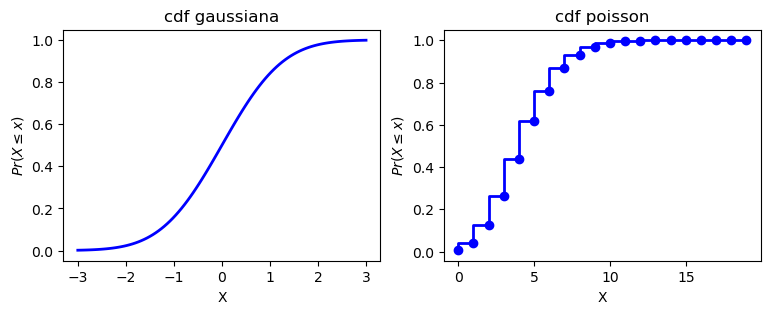
\includegraphics{2.1_funciones_distribucion_densidad_files/figure-pdf/cell-10-output-1.png}

}

\end{figure}

\textbf{Relación entre función de densidad y función de distribución
acumulativa}

Podemos definir la función de densidad de probabilidad, o \emph{pdf},
como la derivada de la cdf

\[
  p(x) \overset{\Delta}{=} \frac{d}{dx}P(x)
\]

Alternativamente, en vez de \(p(x)\) y \(P(x)\) se suele usar, para VA
continuas, \(f(x)\) y \(F(x)\) respectivamente.

Y viceversa: la cdf como la integral de la pdf. Dada la pdf, podemos
calcular la probabilidad de una variable continua en un intervalo finito
como sigue

\[
  \text{Pr}(a <X\leq b) = \int_a^b p(x)dx = P(b) - P(a) \tag{10}
\]

La función de densidad de probabilidad debe satisfacer

\begin{align*}
1)\ &f(x) \geq 0,\ \text{para toda } x,\ -\infty < x < \infty\\
2)\ &\int\_{-\infty}^\infty f(x)\text{d}x = 1
\end{align*}

\begin{center}\rule{0.5\linewidth}{0.5pt}\end{center}

\textbf{Ejemplo con distribución normal}

La pdf de una normal está dada por

\[
  \mathcal{N}(x\mid \mu, \sigma^2)=  p(x) = \frac{1}{\sigma \sqrt{2\pi}} e\left\{\frac{-(x-\mu)^2}{2\sigma^2}\right\} \tag{10}
\]

que es gobernada (es decir, su forma y sus valores quedan completamente
especificados) por \(\mu\), la media o el valor central, y \(\sigma^2\),
llamada la varianza (cuya raíz cuadrada es la desviación estándar
\(\sigma\), y está en las unidades de \(x\) y \(\mu\)).El recíproco de
la varianza es llamado \emph{precisión}, \(\tau=1/\sigma^2\).

En la ecuación (10), el término \(\frac{1}{\sigma \sqrt{2\pi}}\) es una
constante de \emph{normalización}, que asegura que \(p(x)\) sume 1, por
lo que

\[
  \int_{-\infty}^\infty p(x)\text{d}x=1
\]

Las siguientes expresiones se cumplen en (10). El valor esperado de
\(x\) es

\[
  \mathbf{E}[x]=\int_{-\infty}^\infty p(x)x\text{d}x=\mu
\]

Y el valor esperado de \(x^2\)

\[
  \mathbf{E}[x^2] =  \int_{-\infty}^\infty p(x)x\text{d}x^2=\mu^2 + \sigma^2
\]

La varianza está dada por
\(\text{var}[x]=\mathbf{E}[x^2] - \mathbf{E}[x]^2\), por lo que
\(\text{var}[x]=\sigma^2\).

\begin{Shaded}
\begin{Highlighting}[]
\NormalTok{x }\OperatorTok{=}\NormalTok{ np.random.normal(}\DecValTok{4}\NormalTok{, }\DecValTok{3}\NormalTok{, }\DecValTok{10000}\NormalTok{)}
\BuiltInTok{print}\NormalTok{(x.mean())}
\BuiltInTok{print}\NormalTok{(np.mean(x}\OperatorTok{**}\DecValTok{2}\NormalTok{) }\OperatorTok{{-}}\NormalTok{ np.mean(x)}\OperatorTok{**}\DecValTok{2}\NormalTok{)}
\BuiltInTok{print}\NormalTok{(np.var(x))}
\BuiltInTok{print}\NormalTok{(np.std(x).}\BuiltInTok{round}\NormalTok{(}\DecValTok{2}\NormalTok{))}
\end{Highlighting}
\end{Shaded}

\begin{verbatim}
3.9881330919624323
9.149508765663048
9.149508765663052
3.02
\end{verbatim}

En la siguiente figura a la izquierda se representa una variable
aleatoria normal con media 0 y desviación estándar de 1, conocida como
distribución normal estándar, y representada como
\(\mathcal{N}(\mu=0, \sigma = 1)\) o simplemente \(\mathcal{N}(0, 1)\).
Para la densidad de probabilidad normal, en Python usamos
\texttt{scipy.stats.norm.pdf(x,\ loc=0,\ scale=1)}, que nos retorna la
densidad en \texttt{x}. \texttt{norm.}, que nos retorna la densidad en
\texttt{x}.

A la derecha se representa el área equivalente en la cdf, usando
\texttt{scipy.stats.norm.cdf(x,\ loc=0,\ scale=1)}.

\begin{Shaded}
\begin{Highlighting}[]
\CommentTok{\# Setting up plot dimensions}
\NormalTok{fig, axes }\OperatorTok{=}\NormalTok{ plt.subplots(}\DecValTok{1}\NormalTok{, }\DecValTok{2}\NormalTok{, figsize}\OperatorTok{=}\NormalTok{(}\DecValTok{13}\NormalTok{, }\DecValTok{4}\NormalTok{))}

\CommentTok{\# PDF Gaussiana (Normal)}
\NormalTok{x }\OperatorTok{=}\NormalTok{ np.linspace(}\OperatorTok{{-}}\DecValTok{3}\NormalTok{, }\DecValTok{3}\NormalTok{, }\DecValTok{101}\NormalTok{)}
\NormalTok{y }\OperatorTok{=}\NormalTok{ norm.pdf(x, }\DecValTok{0}\NormalTok{, }\DecValTok{1}\NormalTok{)}

\NormalTok{axes[}\DecValTok{0}\NormalTok{].plot(x, y, color}\OperatorTok{=}\StringTok{\textquotesingle{}blue\textquotesingle{}}\NormalTok{, linewidth}\OperatorTok{=}\DecValTok{2}\NormalTok{)}
\NormalTok{axes[}\DecValTok{0}\NormalTok{].set\_title(}\StringTok{\textquotesingle{}pdf gaussiana (normal)\textquotesingle{}}\NormalTok{)}
\NormalTok{axes[}\DecValTok{0}\NormalTok{].set\_ylabel(}\StringTok{\textquotesingle{}p(x)\textquotesingle{}}\NormalTok{)}

\NormalTok{from\_x, to\_x }\OperatorTok{=} \OperatorTok{{-}}\FloatTok{1.5}\NormalTok{, }\FloatTok{1.5}
\NormalTok{sx }\OperatorTok{=}\NormalTok{ np.concatenate([[from\_x], np.arange(from\_x, to\_x, }\FloatTok{0.01}\NormalTok{), [to\_x]])}
\NormalTok{sy }\OperatorTok{=}\NormalTok{ np.concatenate([[}\DecValTok{0}\NormalTok{], norm.pdf(np.arange(from\_x, to\_x, }\FloatTok{0.01}\NormalTok{)), [}\DecValTok{0}\NormalTok{]])}

\NormalTok{axes[}\DecValTok{0}\NormalTok{].fill(sx, sy, color}\OperatorTok{=}\StringTok{\textquotesingle{}\#B3B3FF\textquotesingle{}}\NormalTok{)}
\NormalTok{axes[}\DecValTok{0}\NormalTok{].text(}\OperatorTok{{-}}\DecValTok{1}\NormalTok{, norm.pdf(}\DecValTok{0}\NormalTok{, }\DecValTok{0}\NormalTok{) }\OperatorTok{/} \DecValTok{2}\NormalTok{, }\VerbatimStringTok{r"$\textbackslash{}int\_\{{-}1,5\}\^{}}\SpecialCharTok{\{1.5\}}\VerbatimStringTok{ p(x) dx$"}\NormalTok{, fontsize}\OperatorTok{=}\DecValTok{12}\NormalTok{)}
\NormalTok{axes[}\DecValTok{0}\NormalTok{].text(}\OperatorTok{{-}}\DecValTok{1}\NormalTok{, norm.pdf(}\DecValTok{0}\NormalTok{, }\DecValTok{0}\NormalTok{) }\OperatorTok{/} \DecValTok{3}\NormalTok{, }\StringTok{"= P(1.5) {-} P({-}1.5)"}\NormalTok{, fontsize}\OperatorTok{=}\DecValTok{12}\NormalTok{)}

\CommentTok{\# CDF Gaussiana}
\NormalTok{y\_cdf }\OperatorTok{=}\NormalTok{ norm.cdf(x, }\DecValTok{0}\NormalTok{, }\DecValTok{1}\NormalTok{)}
\NormalTok{axes[}\DecValTok{1}\NormalTok{].plot(x, y\_cdf, color}\OperatorTok{=}\StringTok{\textquotesingle{}blue\textquotesingle{}}\NormalTok{, linewidth}\OperatorTok{=}\DecValTok{2}\NormalTok{)}
\NormalTok{axes[}\DecValTok{1}\NormalTok{].set\_title(}\StringTok{\textquotesingle{}cdf gaussiana\textquotesingle{}}\NormalTok{)}
\NormalTok{axes[}\DecValTok{1}\NormalTok{].set\_xlabel(}\StringTok{\textquotesingle{}X\textquotesingle{}}\NormalTok{)}
\NormalTok{axes[}\DecValTok{1}\NormalTok{].set\_ylabel(}\VerbatimStringTok{r"$Pr(X \textbackslash{}leq x)$"}\NormalTok{)}

\NormalTok{sy\_cdf }\OperatorTok{=}\NormalTok{ np.concatenate([[}\DecValTok{0}\NormalTok{], norm.cdf(np.arange(from\_x, to\_x, }\FloatTok{0.01}\NormalTok{)), [}\DecValTok{0}\NormalTok{]])}
\NormalTok{axes[}\DecValTok{1}\NormalTok{].fill\_between(sx, sy\_cdf, color}\OperatorTok{=}\StringTok{\textquotesingle{}\#B3B3FF\textquotesingle{}}\NormalTok{)}

\NormalTok{plt.show()}
\end{Highlighting}
\end{Shaded}

\begin{figure}[H]

{\centering 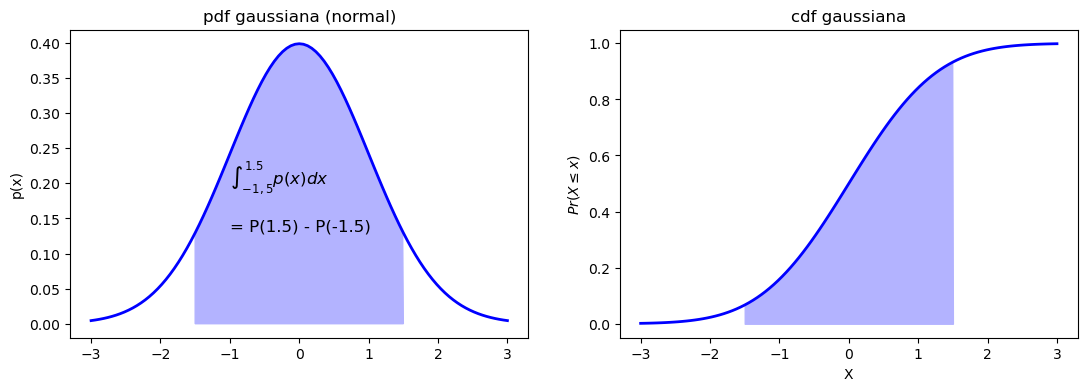
\includegraphics{2.1_funciones_distribucion_densidad_files/figure-pdf/cell-12-output-1.png}

}

\end{figure}

En \texttt{Python}, la función de densidad acumulada CDF para la
distribución normal se obtiene con \texttt{pnorm(x,\ mean,\ sd)}
\texttt{norm.cdf(x,\ mean,\ sd)} en donde \texttt{x} es un vector de
\emph{cuantiles}, que es el, o los, valores en \(x\) para el cual(es)
deseamos obtener su probabilidad (básicamente, un cuantil es la función
inversa de \(P(x)\)).

Para obtener el área sombreada en la anterior figura, usamos
\texttt{norm.cdf(b)-norm.cdf(a)}

\begin{Shaded}
\begin{Highlighting}[]
\NormalTok{norm.cdf(}\FloatTok{1.5}\NormalTok{, }\DecValTok{0}\NormalTok{, }\DecValTok{1}\NormalTok{) }\OperatorTok{{-}}\NormalTok{ norm.cdf(}\OperatorTok{{-}}\FloatTok{1.5}\NormalTok{, }\DecValTok{0}\NormalTok{, }\DecValTok{1}\NormalTok{)}
\end{Highlighting}
\end{Shaded}

\begin{verbatim}
0.8663855974622838
\end{verbatim}

El área que cubre \texttt{pnorm(1.5)} va desde \(-\infty\) a 1.5, y el
área de \texttt{pnorm(-1.5)} va de \(-\infty\) a -1.5. Matemáticamente,
lo anterior se expresaría como

\[
  P(-1.5 < X < 1.5) = \int_{-1.5}^{1.5}\frac{1}{\sigma \sqrt{2\pi}} e\left\{\frac{-(x-\mu)^2}{2\sigma^2}\right\}\text{d}x
\]

En contraste con las \textbf{VA} discretas, la probabilidad de que una
variable continua \(X\in \mathbb{R}\) tome un valor particular,
\(p(X = x)\), es 0. Es como integrar la función de densidad de la
siguiente manera:

\[
  Pr(a \leq X \leq a) = \int_a^b f(x)dx = P(a) - P(a)
\]

Por esta razón, con \(\text{\sf pdf}\) solo calculamos probabilidades en
intervalos.

\begin{center}\rule{0.5\linewidth}{0.5pt}\end{center}

Para VA continuas, las reglas de suma y producto son

\begin{align*}
\text{ \bf{regla de la suma}} \quad\quad &f(x) = \int_y f(x,y)\text{d}y \\
\text{ \bf{regla del producto}}\quad\quad &f(x, y) = f(y|x)f(x)
\end{align*}

En donde \(f(x)\) es la función de probabilidad marginal, y se integra
\emph{con respecto a} \(y\). Lo mismo si queremos encontrar la marginal
de \(y\) tenemos que integrar \(f(x,y)\) \emph{con respecto a} \(x\).

\hypertarget{funciuxf3n-acumulada-de-probabilidad-conjunta}{%
\subsection{Función acumulada de probabilidad
conjunta}\label{funciuxf3n-acumulada-de-probabilidad-conjunta}}

Sean \(X_1, X_2\) variables aleatorias continuas con función de
distribución conjunta \(F(x_1, x_2)\). La función de distribución
bivariante \(F(x_1, x_2)\) es

\[
  F(x_1, x_2) = P(X_1 \leq x_1, X_2 \leq x_2),\quad -\infty < x_1 < \infty, -\infty < x_2<\infty
\]

Si existe una función no negativa \(f(x_1, x_2)\), se obtiene

\begin{align*}
F(x_1, x_2) = \int*{-\infty}^{x_2} \int_{-\infty}^{x_1} f(t_1, t_2)\text{d}t_1\text{d}t_2
\end{align*}

Para toda \(-\infty < x_1<\infty, -\infty < x_2<\infty\). En donde
\(t_1, t_2\) son solo variables de integración.

Satisfacen

\begin{align*}
1. &f(x_1, x_2)\geq 0\quad \text{para toda }x_1, x_2\\
2. &\int_{-\infty}^\infty f(x_1, x_2) \text{d}x_1\text{d}x_2= 1
\end{align*}

\textbf{Ejemplos}

\begin{enumerate}
\def\labelenumi{\arabic{enumi}.}
\tightlist
\item
  Dada \(f(y) = cy^2,\ 0 \leq y \leq 2\) y \(f(y)=0\) en cualquier otra
  parte, encuentre el valor de \(c\) para el cuál \(f(y)\) es una
  función de densidad válida.
\end{enumerate}

\begin{quote}
\emph{Solución}
\end{quote}

\begin{quote}
Para obtener \(c\), requerimos un valor tal que se cumpla
\end{quote}

\begin{quote}
\[
 F(y) = \int_{-\infty}^\infty f(y)\text{d}y = 1
\]

Lo que nos da

\[
 F(y) = \int_0^2 cy^2\text{d}y=\frac{cy^3}{3} \Bigg|_0^2=\frac{8}{3}c
\]

Sustituyendo \(\frac{8}{3}c=1\) nos da que \(c=3/8\).
\end{quote}

\begin{enumerate}
\def\labelenumi{\arabic{enumi}.}
\setcounter{enumi}{1}
\tightlist
\item
  Encontrar \(P(1\leq Y \leq 2)\) para la función del ejemplo 1, también
  encontrar \(P(1< Y < 2)\)
\end{enumerate}

\begin{quote}
\emph{Solución}
\end{quote}

\begin{quote}
Dado que ya encontramos el valor de que satisface
\(F(y) = \int_{-\infty}^\infty f(y)\text{d}y = 1\), la sustituimos.

\[
 P(1\leq Y \leq 2) = \int_1^2 f(y)\text{d}y= \frac{3}{8}\int_1^2 y^2\text{d}y=7/8
\]
\end{quote}

\begin{enumerate}
\def\labelenumi{\arabic{enumi}.}
\setcounter{enumi}{2}
\tightlist
\item
  Como una medida de inteligencia, a unos ratones se les toma el tiempo
  que tardan para pasar por un laberinto para llegar a una recompensa
  (alimento). El tiempo en segundos necesario para cualquier ratón es
  una variable aleatoria \(Y\) con función de densidad dada por
\end{enumerate}

\[
  f(y) = \begin{cases}
    \frac{b}{y^2},\ &y\geq b\\
    0,\ &\text{en cualquier otro punto}
  \end{cases}
\]

En donde \(b\) es el tiempo mínimo posible para recorrer el laberinto.
Demostrar que \(f(y)\) tiene las propiedades de una función de densidad.

\begin{quote}
\emph{Solución}
\end{quote}

\begin{quote}
Dado que \(b\) es un tiempo, no puede ser negativo. Además, \(f(y)\)
tiene el término cuadrático \(y^2\), que tampoco puede ser negativo, por
lo que \(f(y) \geq 0\).

El mínimo valor que puede tener \(y\) es \(b\). Por lo tanto

\begin{align*}
F(y) &= \int\_{b}^\infty \frac{b}{y^2}\text{d}y= 1\\  
 &= \frac{by^{-2+1}}{-2+1}\Bigg|\_b^\infty=-\frac{b}{y}\Bigg|\_b^\infty=0-\left(-\frac{b}{b}\right)=1
\end{align*}
\end{quote}

\begin{enumerate}
\def\labelenumi{\arabic{enumi}.}
\setcounter{enumi}{3}
\tightlist
\item
  En el ejemplo 1 determinamos que \(f(y)=(3/8)y^2\) para
  \(0\leq y \leq 2, f(y)=0\) en cualquier otra parte. Si la variable
  \(Y\) tiene esta función de densidad, encontrar
  \(\mu=\mathbf{E}[Y], \sigma^2=\text{var}[Y]\), recordando que
  \(\text{var}[x]=\mathbf{E}[x^2]-(\mathbf{E}[x])^2\).
\end{enumerate}

\begin{quote}
\emph{Solución}
\end{quote}

\begin{quote}
\begin{align*}
\mathbf{E}[Y] &= \int_{-\infty}^\infty yf(y)\text{d}y= \int_{-\infty}^\infty y\frac{3y^2}{8}\text{d}y = \frac{3}{8}\cdot\frac{1}{4}y^4 \Bigg|_0^2=1.5\\
\text{para } &\mathbf{E}[Y^2]\quad \text{se obtiene}\\
\mathbf{E}[Y^2] &= \int_{-\infty}^\infty y^2f(y)\text{d}y= \int\_{-\infty}^\infty y^2\frac{3y^2}{8}\text{d}y = \frac{3}{8}\cdot\frac{1}{5}y^5 \Bigg|\_0^2=2.4\\
\text{por }&\text{lo que}\\
\text{var}[x]&=\mathbf{E}[x^2]-(\mathbf{E}[x])^2 = 2.4 - 1.5^2 = 0.15
\end{align*}
\end{quote}

\begin{enumerate}
\def\labelenumi{\arabic{enumi}.}
\setcounter{enumi}{4}
\tightlist
\item
  Una partícula radiactiva se localiza en un cuadrado con lados de
  longitud 1. Denotar como \(Y_1, Y_2\) las coordenadas de la ubicación
  de la partícula. Un modelo razonable para el histograma de frecuencia
  relativa para \(Y_1, Y_2\) es la función bivariante de densidad
\end{enumerate}

\[
  f(y_1, y_2) = \begin{cases}
  1,\quad & 0 \leq y_1 \leq 1, 0 \leq y_2 \leq 1\\
  0, \quad & \text{en cualquier otro punto}
  \end{cases}
\]

Econtrar \(F(y_1=0.2, y_2=0.4)\), que es lo mismo que encontrar la
probabilidad \(P(y_1<0.2, y_2<0.4)\).

\begin{quote}
\emph{Solución}
\end{quote}

\begin{quote}
\begin{align}
F(y*1=0.2, y_2=0.4)%
&= \int_{-\infty}^{0.4} \int_{-\infty}^{0.2} f(y_1, y_2)\text{d}y_1\text{d}y_2 \\
&= \int_{-\infty}^{0.4} \int_{-\infty}^{0.2} (1)\text{d}y_1\text{d}y_2 \\
&= \int_{-\infty}^{0.4} \left(\int_{-\infty}^{0.2} \text{d}y_1\right)\text{d}y_2\\
&= \int_{-\infty}^{0.4} \Bigg( y_1\Big|\_0^{0.2} \Bigg)\text{d}y_2\\
&= \int_{-\infty}^{0.4} 0.2 \text{d}y_2 = 0.2y_2\Big|\_0^{0.4} = 0.08
\end{align}
\end{quote}

\begin{enumerate}
\def\labelenumi{\arabic{enumi}.}
\setcounter{enumi}{5}
\tightlist
\item
  Sea
\end{enumerate}

\begin{center}\rule{0.5\linewidth}{0.5pt}\end{center}

\[
  f(y_1, y_2) = \begin{cases}
    2y_1\quad 0 \leq y_1 \leq, 0 \leq y_2 \leq\\
    0,\quad \text{en otro punto}
  \end{cases}
\]

\begin{enumerate}
\def\labelenumi{\alph{enumi})}
\tightlist
\item
  Obtener las funciones de densidad marginal \(f(y_1)\) y \(f(y_2)\).
\item
  Obtener la función condicional \(f(y_1 | y_2)\)
\item
  Demostrar si las variables \(Y_1, Y_2\) son independientes.
\end{enumerate}

\begin{quote}
\emph{Solución}
\end{quote}

\begin{quote}
\begin{enumerate}
\def\labelenumi{\alph{enumi})}
\tightlist
\item
  La marginal de \(f(y_1)\) se obtiene aplicando la regla
\end{enumerate}

\[
 f(x) = \int_{-\infty}^\infty f(x, y)\text{d}y
\]

Notar que para obtener la marginal de la variable \(x\) se integra la
función conjunta con respecto a \(y\). Esto significa que trataremos a
\(x\) como \emph{constante}. En este caso, como tenemos \(y_1, y_2\) en
vez de \(x, y\), la marginal sería

\[
 f(y_1)= \int_{-\infty}^\infty f(y_1, y_2)\text{d}y_2=\int_{0}^12y_1\text{d}y_2
\]

Y trataremos a \(y_1\) como constante, y usamos la regla
\(\int \text{d}x=x\)

\[
 f(y_1)=\int_{0}^12y_1\text{d}y_2=2y_1\int_{0}^1\text{d}y_2=2y_1\left(y_2\Big|_0^1\right)=2y_1
\]

Para \(f(y_2)\) seguimos un razonamiento similar.

\[
 f(y_2)= \int_{-\infty}^\infty f(y_1, y_2)\text{d}y_1=\int_{0}^12y_1\text{d}y_1
\]

Pero ahora integramos con respecto a \(y_1\). Aplicamos la regla
\(\int x^n \text{d}x=\frac{x^{n+1}}{n+1}\)

\[
 f(y_2)=\int_{0}^12y_1\text{d}y_1=2\frac{y_1^2}{2}\Big|_0^1=y_1^2\Big|_0^1=1
\]

La marginal de \(y_2\) es una constante. b) La función condicional se
puede obtener con la siguiente regla

\[
 f(x|y) = \frac{f(x, y)}{f(x)}
\]

Por lo que para obtener \(f(y_1|y_2)\) necesitamos la densidad conjunta
(que ya tenemos), y la marginal de \(f(y_2)\), que ya tenemos también.

\[
 f(y_1|y_2) = \frac{f(y_1, y_2)}{f(y_2)} = \frac{2y_1}{1}=2y_1
\]

La condicional sigue siendo la conjunta porque la marginal es una
constante. c) La demostración de que las variables son independientes es
trivial siguiendo la regla: \(x,y\) son independientes \emph{si y solo
si} \(f(x,y)=f(x)f(y)\)
\end{quote}

\begin{enumerate}
\def\labelenumi{\arabic{enumi}.}
\setcounter{enumi}{6}
\tightlist
\item
  Sea la función de densidad conjunta
\end{enumerate}

\begin{center}\rule{0.5\linewidth}{0.5pt}\end{center}

\[
  f(y_1, y_2) = \begin{cases}
    e^{-(y_1 + y_2)}\quad y_1>0, y_2>0\\
    0,\quad \text{en otro punto}
  \end{cases}
\]

\begin{enumerate}
\def\labelenumi{\alph{enumi})}
\item
  Encontrar \(f(y_1)\) y \(f(y_2)\).
\item
  ¿Cuál es la probabilidad \(P(1 < Y_1 < 2.5)\) y \(P(1 < Y_2 < 2.5)\)?
\item
  Para cualquier \(Y_2>0\), ¿cuál es la función \(f(y_1|y_2)\)?
\end{enumerate}

\begin{quote}
\emph{Solución}
\end{quote}

\begin{quote}
\begin{enumerate}
\def\labelenumi{\alph{enumi})}
\tightlist
\item
  Primero notar que tanto \(y_1\) como \(y_2\) están en el intervalo
  \((0, \infty)\), por lo que esos son sus límites de integración.
  Formalmente, lo correcto sería encontrar el límite de la integral
\end{enumerate}

\[
 f(y_1)=\lim_{t\rightarrow \infty}\int_{-\infty}^{\infty}f(y_1,y_2)\text{d}y_2
\]

Sin embargo, \emph{informalmente} sabemos que \(e^{-\infty}=0\).
Aplicamos la regla de los exponentes \(a^na^m=a^{n+m}\) a
\(e^{-(y_1+y_2)}=e^{-y_1}e^{-y_2}\)

\[
 f(y_1)=\int_{-\infty}^{\infty}f(y_1,y_2)\text{d}y_2=\int_0^{\infty}e^{-y_1}e^{-y_2}\text{d}y_2=e^{-y_1}\int_0^{\infty}e^{-y_2}\text{d}y_2
\]

Para integrar lo anterior, consideramos la siguiente regla
\(\int e^{-u}du=-e^{-u}\)

\[
 f(y_1) = e^{-y_1}\int_0^{\infty}e^{-y_2}\text{d}y_2=e^{-y_1}\left(-e^{-y_2}\Big|_0^\infty\right)=e^{-y_1}\left(-(e^\infty-e^0)\right)=\cdots=e^{-y_1}
\]

El mismo razonamiento para \(f(y_2)\) nos da un resultado similar
\end{quote}

\[
  f(y_2)=\int_{-0}^{\infty}e^{-(y_1+y_2)}\text{d}y_1=\cdots=e^{-y_2}
\]

\begin{quote}
\begin{enumerate}
\def\labelenumi{\alph{enumi})}
\setcounter{enumi}{1}
\tightlist
\item
  Para obtener esta probabilidad (acumulada) necesitamos la regla
\end{enumerate}
\end{quote}

\begin{quote}
\[
 P(a < X < b)=\int_a^b f(x)\text{d}x
\]

En donde \(f(x)\) en nuestro caso corresponde a las marginales
\(f(y_1)=e^{-y_1}, f(y_2)=e^{-y_2}\)

\[
 P(1<Y_1<2.5)=\int_1^{2.5}e^{-y_1}\text{d}y_1=-e^{-y_1}\Big|_1^{2-5}=-\left(e^{-2.5}-e^{-1}\right)=\cdots=0.285
\]

Un razonamiento similar aplica para la segunda parte del ejercicio.
\end{quote}

\begin{quote}
\begin{enumerate}
\def\labelenumi{\alph{enumi})}
\setcounter{enumi}{2}
\tightlist
\item
  Usamos la regla del producto ya revisada: \(f(x|y)=f(x,y)/f(y)\). La
  conjunta es \(f(y_1,y_2)=e^{-(y_1+y_2)}=e^{-y_1}e^{-y_2}\) y la
  marginal \(f(y_2)=e^{-y_2}\)
\end{enumerate}

\[
 f(y_1|y_2)=\frac{e^{-y_1}e^{-y_2}}{e^{-y_2}}=e^{-y_1},\quad \text{para todo } y_2>0
\]

Un razonamiento similar aplica a \(f(y_2|y_2)\).
\end{quote}

\begin{enumerate}
\def\labelenumi{\arabic{enumi}.}
\setcounter{enumi}{7}
\tightlist
\item
  Ejemplo de una normal
\end{enumerate}

La temperatura promedio de una máquina es de 37°C, con una desviación
estándar medida de 1.5. Suponiendo que la distribución de la temperatura
puede ser aproximada por una normal, ¿qué tan probable es encontrar una
temperatura de 35 o menos?

\begin{quote}
\emph{Solución}
\end{quote}

\begin{quote}
Queremos hallar la probabilidad \(P(X<35)\) sabiendo que
\(X\sim \mathcal{N}(\mu=37, \sigma=1.5)\). Es decir

\[
 P(X<35)=\int_{0}^{35}\frac{1}{1.5 \sqrt{2\pi}} e\left\{\frac{-(x-37)^2}{2(1.5)^2}\right\}\text{d}x
\]
\end{quote}

\begin{Shaded}
\begin{Highlighting}[]
\CommentTok{\# Setting up plot dimensions}
\NormalTok{fig, axes }\OperatorTok{=}\NormalTok{ plt.subplots(}\DecValTok{1}\NormalTok{, }\DecValTok{2}\NormalTok{, figsize}\OperatorTok{=}\NormalTok{(}\DecValTok{13}\NormalTok{, }\DecValTok{4}\NormalTok{))}

\CommentTok{\# PDF}
\NormalTok{x }\OperatorTok{=}\NormalTok{ np.linspace(}\DecValTok{30}\NormalTok{, }\DecValTok{45}\NormalTok{, }\DecValTok{101}\NormalTok{)}
\NormalTok{y }\OperatorTok{=}\NormalTok{ norm.pdf(x, }\DecValTok{37}\NormalTok{, }\FloatTok{1.5}\NormalTok{)}

\NormalTok{axes[}\DecValTok{0}\NormalTok{].plot(x, y, color}\OperatorTok{=}\StringTok{\textquotesingle{}blue\textquotesingle{}}\NormalTok{, linewidth}\OperatorTok{=}\DecValTok{2}\NormalTok{)}
\NormalTok{axes[}\DecValTok{0}\NormalTok{].set\_title(}\StringTok{\textquotesingle{}pdf\textquotesingle{}}\NormalTok{)}
\NormalTok{axes[}\DecValTok{0}\NormalTok{].set\_ylabel(}\StringTok{\textquotesingle{}p(x)\textquotesingle{}}\NormalTok{)}

\NormalTok{from\_x, to\_x }\OperatorTok{=} \DecValTok{30}\NormalTok{, }\DecValTok{35}
\NormalTok{sx }\OperatorTok{=}\NormalTok{ np.concatenate([[from\_x], np.arange(from\_x, to\_x, }\FloatTok{0.01}\NormalTok{), [to\_x]])}
\NormalTok{sy }\OperatorTok{=}\NormalTok{ np.concatenate([[}\DecValTok{0}\NormalTok{], norm.pdf(np.arange(from\_x, to\_x, }\FloatTok{0.01}\NormalTok{), }\DecValTok{37}\NormalTok{, }\FloatTok{1.5}\NormalTok{), [}\DecValTok{0}\NormalTok{]])}

\NormalTok{axes[}\DecValTok{0}\NormalTok{].fill(sx, sy, color}\OperatorTok{=}\StringTok{\textquotesingle{}\#B3B3FF\textquotesingle{}}\NormalTok{)}
\NormalTok{axes[}\DecValTok{0}\NormalTok{].text(}\DecValTok{35} \OperatorTok{+} \DecValTok{1}\NormalTok{, norm.pdf(}\DecValTok{35}\NormalTok{, }\DecValTok{37}\NormalTok{, }\FloatTok{1.5}\NormalTok{), }\StringTok{\textquotesingle{}x=35\textquotesingle{}}\NormalTok{, fontsize}\OperatorTok{=}\DecValTok{12}\NormalTok{)}

\CommentTok{\# CDF}
\NormalTok{y\_cdf }\OperatorTok{=}\NormalTok{ norm.cdf(x, }\DecValTok{37}\NormalTok{, }\FloatTok{1.5}\NormalTok{)}
\NormalTok{axes[}\DecValTok{1}\NormalTok{].plot(x, y\_cdf, color}\OperatorTok{=}\StringTok{\textquotesingle{}blue\textquotesingle{}}\NormalTok{, linewidth}\OperatorTok{=}\DecValTok{2}\NormalTok{)}
\NormalTok{axes[}\DecValTok{1}\NormalTok{].set\_title(}\StringTok{\textquotesingle{}cdf\textquotesingle{}}\NormalTok{)}
\NormalTok{axes[}\DecValTok{1}\NormalTok{].set\_xlabel(}\StringTok{\textquotesingle{}X\textquotesingle{}}\NormalTok{)}
\NormalTok{axes[}\DecValTok{1}\NormalTok{].set\_ylabel(}\VerbatimStringTok{r"$Pr(X \textbackslash{}leq x)$"}\NormalTok{)}

\NormalTok{sy\_cdf }\OperatorTok{=}\NormalTok{ np.concatenate([[}\DecValTok{0}\NormalTok{], norm.cdf(np.arange(from\_x, to\_x, }\FloatTok{0.01}\NormalTok{), }\DecValTok{37}\NormalTok{, }\FloatTok{1.5}\NormalTok{), [}\DecValTok{0}\NormalTok{]])}
\NormalTok{axes[}\DecValTok{1}\NormalTok{].fill\_between(sx, sy\_cdf, color}\OperatorTok{=}\StringTok{\textquotesingle{}\#B3B3FF\textquotesingle{}}\NormalTok{)}

\NormalTok{axes[}\DecValTok{1}\NormalTok{].text(}\DecValTok{35} \OperatorTok{+} \DecValTok{1}\NormalTok{, norm.cdf(}\DecValTok{35}\NormalTok{, }\DecValTok{37}\NormalTok{, }\FloatTok{1.5}\NormalTok{), }\StringTok{\textquotesingle{}x=35\textquotesingle{}}\NormalTok{, fontsize}\OperatorTok{=}\DecValTok{12}\NormalTok{)}

\NormalTok{plt.show()}
\end{Highlighting}
\end{Shaded}

\begin{figure}[H]

{\centering 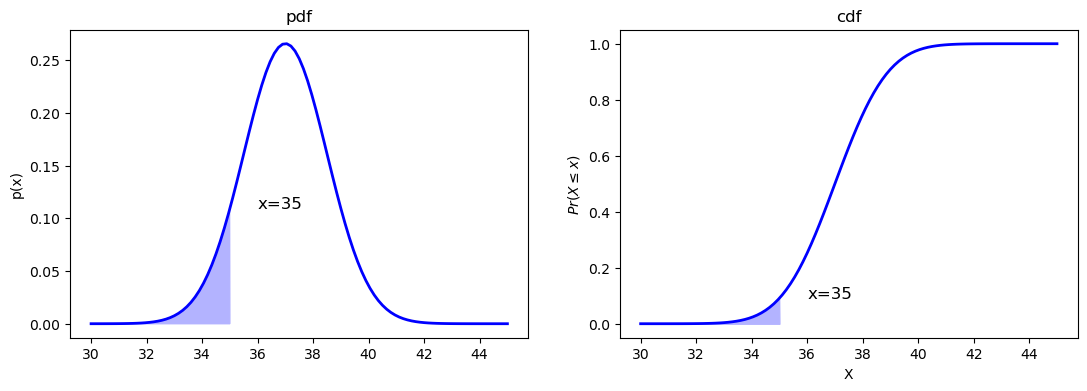
\includegraphics{2.1_funciones_distribucion_densidad_files/figure-pdf/cell-14-output-1.png}

}

\end{figure}

El área se obtiene en Python con el siguiente código, que usa la cdf
normal, \texttt{pnorm}. El primer argumento es el \emph{cuantil}
\texttt{q}, el valor en el eje \emph{x} del cual queremos saber el área
bajo la curva.

\begin{Shaded}
\begin{Highlighting}[]
\NormalTok{norm.cdf(}\DecValTok{35}\NormalTok{, }\DecValTok{37}\NormalTok{, }\FloatTok{1.5}\NormalTok{)}
\CommentTok{\# ¿cuál sería la probabilidad de tener 37 o menos?}
\end{Highlighting}
\end{Shaded}

\begin{verbatim}
0.09121121972586788
\end{verbatim}

Equivalentemente, en Python se puede integrar la pdf con integración
numérica

\begin{Shaded}
\begin{Highlighting}[]
\ImportTok{from}\NormalTok{ scipy.integrate }\ImportTok{import}\NormalTok{ quad}

\CommentTok{\# Define the function to integrate}
\KeywordTok{def}\NormalTok{ f(x, mean, sd):}
    \ControlFlowTok{return}\NormalTok{ norm.pdf(x, mean, sd)}

\CommentTok{\# Perform numerical integration}
\NormalTok{result, error }\OperatorTok{=}\NormalTok{ quad(f, }\DecValTok{0}\NormalTok{, }\DecValTok{35}\NormalTok{, args}\OperatorTok{=}\NormalTok{(}\DecValTok{37}\NormalTok{, }\FloatTok{1.5}\NormalTok{))}

\BuiltInTok{print}\NormalTok{(}\SpecialStringTok{f"Result of the integration: }\SpecialCharTok{\{}\NormalTok{result}\SpecialCharTok{\}}\SpecialStringTok{"}\NormalTok{)}
\BuiltInTok{print}\NormalTok{(}\SpecialStringTok{f"Estimated error: }\SpecialCharTok{\{}\NormalTok{error}\SpecialCharTok{\}}\SpecialStringTok{"}\NormalTok{)}
\end{Highlighting}
\end{Shaded}

\begin{verbatim}
Result of the integration: 0.09121121972586801
Estimated error: 6.708159657636305e-10
\end{verbatim}



\end{document}
